\chapter{Literature review}%
\label{ch:lit-review}

% TODO: introduction or out
In the past,
computational tools were mainly used to explain chemical reactions after experiments had already been done.
However,
with the recent development of software and hardware technologies,
these tools have become more reliable and can now be used to provide valuable insights and even make predictions~\cite{Ahn_2019}.

% TODO: introduction or out
Modern technology has made it easier and more affordable to access high-performance computing hardware and efficient quantum chemical modeling software.
This has allowed researchers to use quantum chemical reaction modeling techniques more widely in chemical research,
especially in the field of organic and organometallic catalysis.

% TODO: introduction or out
Initially,
computer models were used to explain experimental observations,
but with the development of density functional theory (DFT),
it became possible to model molecules of realistic size and complexity with little to no structural simplifications.
This has enabled researchers to use these models to optimize and even predict new reactions that would not be possible with purely experimental approaches.

% TODO: introduction or out
\citeauthor{Ahn_2019} highlighted several studies that used computational predictions to explain unexpected reactivities or provide mechanistic insights for organic and organometallic reactions,
which led to improved experimental results.
According to the authors,
the key to these successful applications is combining theory and experiment,
which allows for the combination of empirical knowledge with precise computed values\cite{Ahn_2019}.

% TODO: introduction or out
Computational models can be used to virtually optimize novel or practical catalysts and develop new reactions before they are tested in the lab.
This can save time and effort compared to experimenting.
Virtual screening is becoming more popular as a way to find molecules and materials with desirable properties.
However,
automated optimization techniques are not always successful and often require classical chemical logic and conventional strategies of reaction design.
Density Functional Theory (DFT) calculations can provide energies and structures of intermediates that may not be accessible experimentally,
and can also allow for a qualitative examination of the electronic structure that is responsible for the numerical result.
This can help to develop general concepts that can be applied to a whole class of reactions.

% TODO: my text below

% TODO: introduction or out
For centuries,
chemists have seeked to understand the underpinnings of chemical reactions,
and the mechanisms by which they proceed~\cite{Armstrong_1887}.
It is crucial to understand the mechanisms of reaction in order to maximize the efficiency of a reaction
and to minimize unwanted side reactions.
Mechanistic insights can help us predict and control the course of a reaction,
allowing us to tailor a reaction to a particular end goal.
By better understanding reaction mechanisms,
we can design safer,
more efficient processes,
and more powerful synthetic tools.

% TODO: introduction or out
In order to accomplish this,
many concepts and techniques were devised.
Reactivity descriptors,
such as
Hammond's postulate~\cite{Hammond_1955,Cremer_2012,HammondPrinciple} or
Woodward-Hoffmann rules~\cite{Havinga_1961,Woodward_1965,Dewar_1966,Zimmerman_1966,Woodward_1969,Nobel_1981},
aid in predicting the course of a reaction,
as does frontier orbital theory~\cite{Fukui_1952,Brown_2013}.

% TODO: introduction or out
\subsection{Bell-Evans-Polanyi principle}
The Bell-Evans-Polanyi (BEP) principle is a fundamental principle in the study
of chemical reactions.
It states that the more exothermic reactions usually have to overcome lower
reaction barriers and are therefore faster.
It is customary to successfully extend this concept to exergonic reactions.
Notwithstanding,
since the largest contribution is the electronic energy,
it is reasonably
safe to apply the BEP principle (and Hammer's postulate,
as we will see later)
using electronic energies in the context of quantum chemistry calculations.

% TODO: introduction or out
All these descriptors have in common a theoretical ground.
With advances in computing technology,
however,
the power of the computational chemistry has become more and more apparent in recent years.
The use of computational techniques allows the accurate prediction of reaction mechanisms,
as well as detailed insight into potential reaction pathways;
possibly previously unknown synthetic pathways can be successfully explored.
In addition,
the usefulness of computational chemistry extends from organic and inorganic synthesis to biochemistry,
allowing the prediction of reaction mechanisms even in complex systems~\cite{Klippenstein_2014}.
By utilizing these powerful computational techniques,
we can better understand the mechanisms of reaction in the laboratory,
and allow us to come up with targeted,
effective reactions.

% TODO: extra thing to add at the end
% TODO: introduction or out
Computer modeling of chemical reactions is becoming more and more popular among researchers,
and it is expected that its usefulness in predicting reactions will continue to grow in the near future~\cite{Ahn_2019}.

% TODO: introduction or out
\citeauthor{Ahn_2019} highlight how computational studies can be used to design new chemical reactions,
by performing calculations that can be used to predict new reactions,
which is different from their traditional role of just explaining what has already been observed in experiments~\cite{Ahn_2019}.
They emphasize, however,
that it is not yet possible to routinely or automatically design new chemical reactions using computers~\cite{Ahn_2019}.
We hope this changes soon.

% TODO: where to put this? appendix?
\section{Intramolecular and substitutional effects:
  a key step to understand enzyme-like catalysis}

Despite the great advancements in the developments of artificial enzymes~\cite{Breslow_1995},
the synthetic reproduction of the reaction rate accelerations attained by
natural enzymes is far from being reached.
To get there,
we will need a more detailed comprehension of the ways enzymes
work at the molecular level~\cite{Catalysis_in_Chemistry_and_Enzymology}.
Much effort has been put in this direction,
with at least six Nobel Prizes
awarded in this and related areas~\cite{Nobel_1929,Nobel_1946,Nobel_1957,Nobel_1975,Nobel_1997,Nobel_2013}.
These progresses show that the main source of acceleration in
enzymatic reactions is to be found in the events that accompany the
enzyme-substrate complex formation that leads to bond breaking and
formation~\cite{Catalysis_in_Chemistry_and_Enzymology}.
These events induce conformational changes in both substrate and enzyme,
which
enhances the interactions in the active site~\cite{Fischer_1890,Fischer_1894,Koshland_1958,Dafforn_1971,Kirby_1996}.
PICTURES OF REPRESENTATIVE SCHEMES.\@
As a result,
substrate active centers adequately orient themselves towards
their counterparts in the active site,
which leads to
i.\ a decrease in stability of the ground state (if compared with the
free substrate state),
ii.\ a lowering of the transition state energy (if compared with the
non-catalyzed reaction),
iii.\ energy relaxation through the formation of intermediates and
products.

These driving forces are also found in intramolecular reactions (\cref{fig:reacoes-intramoleculares}).
%
\begin{figure}[hbtp]
	\centering
	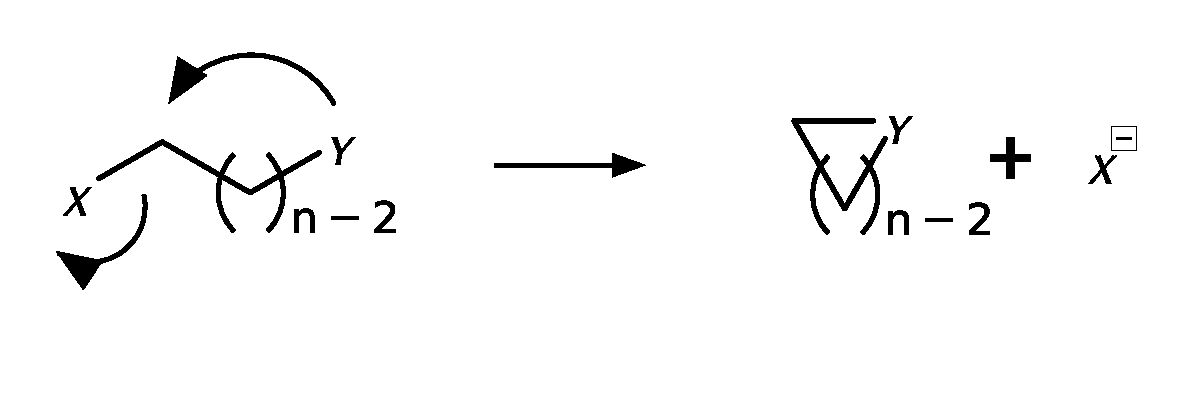
\includegraphics[width=.6\textwidth]{figures/reacao-intramolecular}
	\caption[Typical scheme of an intramolecular reactions]{
		Reaction scheme of a typical intramolecular reaction,
		whose products or
		intermediates are often cycles.
		Smaller rings ($n \le 4 $)
		tend to be disfavored by enthalpy,
		while larger rings ($n \ge 7 $)
		have less probable formation due to entropy.}%
	\label{fig:reacoes-intramoleculares}
\end{figure}
%
In fact,
the similarities between monomolecular enzymatic processes and
intramolecular reactions have been already recognized~\cite{Nilsson_1933,Bruice_1960b,Jung_1990}.
Despite the limitations of using intramolecular reactions as a model for
enzymatic reactions,
it is natural to suppose that the detailed understanding
of enzyme catalysis has,
as a prerequisite,
the ability to understand the
related processes in simpler systems.~\cite{Kirby_1972}.

Mechanisms were validated on the basis of the agreement relative to respective experimental results~\cite{Kirby_1972,Jung_2005}.
The relevant thermochemistry was calculated in room temperature and atmospheric pressure (298.15~K e 1~atm).
Particular details concerning the intramolecular effects of geminal and
vicinal disubstitutions can be found in~\cref{ch:gem-vic-disubstitions}.
